The Deep Residual Channel Attention Network (DRCAN) proposed by Zhang et al. \cite{zhangImageSuperResolutionUsing2018}, 
the channel attention mechanism is introduced to single image super resolution.
Channel Attention enables the network to dynamically assess which feature maps / channels are more important or need more refinement.
This is achieved by processing the globally pooled average of the feature maps using a lightweight network
and then reweighing the feature maps based thereon.

\begin{figure}[h!]
    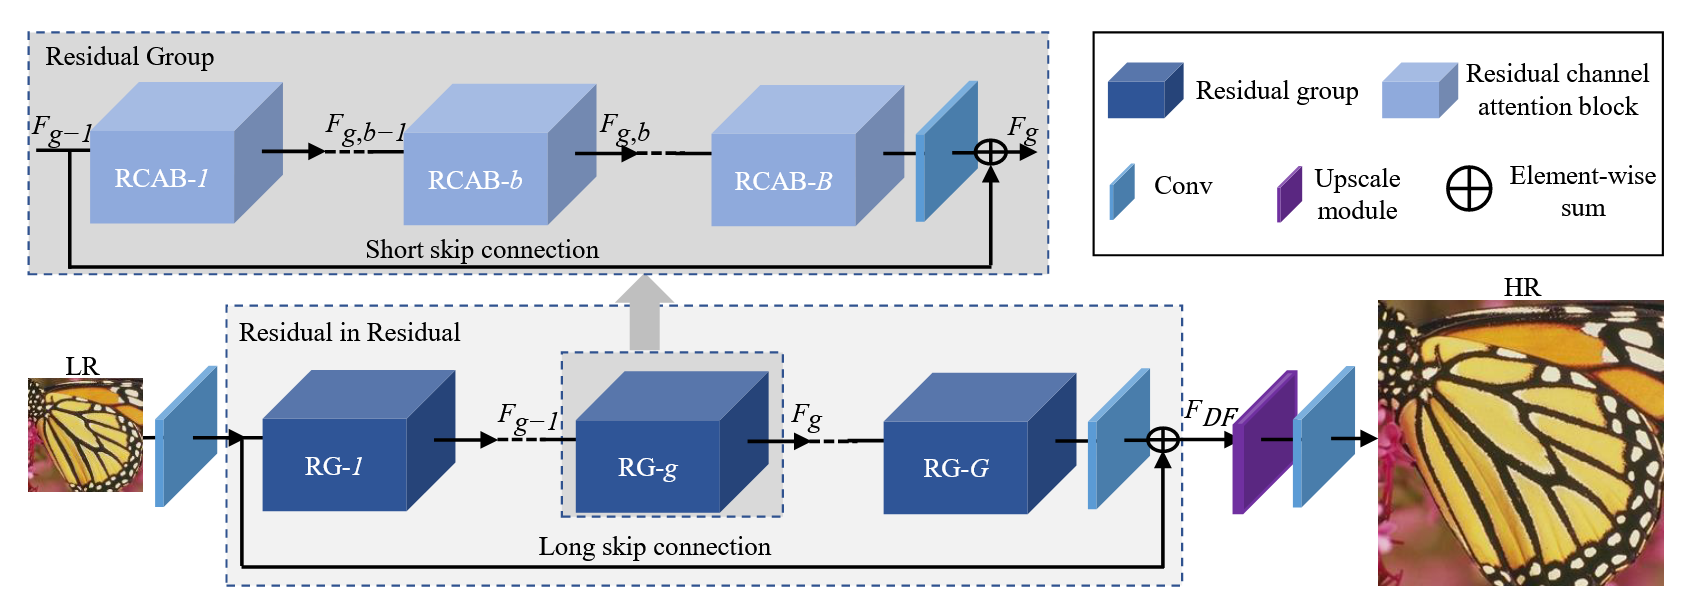
\includegraphics[width=0.9\textwidth]{models/sisr/imgs/drcan_model.png}
    \caption{Image taken from \cite{zhangImageSuperResolutionUsing2018}, DRCAN model architecture.}
    \label{fig:drcan_model}
\end{figure}

The overall model architecture is depicted in figure \ref{fig:drcan_model}.
The input image $X$ is first processed via an initial convolutional layer

    $$ F_0 = C(3, 64, \text{kernel-size}=3, \text{padding}=1)(X) ~. $$

The following convolutional layers used in the architecture of the DRCAN are of the form    

    $$ C = C(64, 64, \text{kernel-size}=3, \text{padding}=1, \text{padding-mode}=\text{zero}) ~, $$

that is $64$ ingoing feature maps processed by $64$ quadratic kernels of size $3 \times 3$ with zero-padding of size $1$, 
so that feature map sizes are conserved throughout the model.
The inial features $F_0$ are then further processed by a network with a residual in residual architecture

    $$ F_{1} = H_{D}(F_0) ~. $$

For low-frequency features to bypass the deep feature extraction, 
a residual connection is used before the upsampling is performed

    $$F_2 = F_0 + F_1 ~.$$

The final features $F_2$ are then upsampled using transposed convolutional layers. \newline
The $H_{RIR}$ network is composed of $10$ Residual Groups followed by a final convolutional layer, 
that is 

    $$ H_{D} = C \circ H_{RG} \circ ... \circ H_{RG} ~.$$

The Residual Groups (RG) are again composed of $20$ Residual Channel Attention Blocks followed as well by a convolutional layer,
the structure is encapsuled in a residual connection

    $$ H_{RG} = R \big ( C \circ H_{RCAB} \circ ... \circ H_{RCAB} \big) ~.$$

\begin{figure}[h!]
    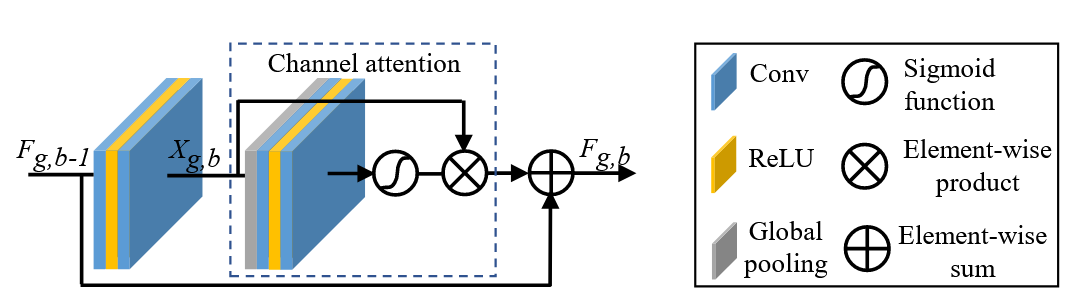
\includegraphics[width=0.9\textwidth]{models/sisr/imgs/drcan_rcab.png}
    \caption{Image taken from \cite{zhangImageSuperResolutionUsing2018}, architecture of RCAB module.}
    \label{fig:drcan_rcab}
\end{figure}

The Residual Channel Attention Block (RCAB) depicted in figure \ref{fig:drcan_rcab}, 
is made up of two convolutional layer, 
with a ReLU activation function in between, 
followed by a channel attention module,
the output is then added back to the input again via a residual connection

    \begin{equation} \label{eq:rcab}
        H_{RCAB} = R \big( H_{CA} \circ C \circ \text{ReLU} \circ C \big) ~.
    \end{equation}

\begin{figure}[h!]
    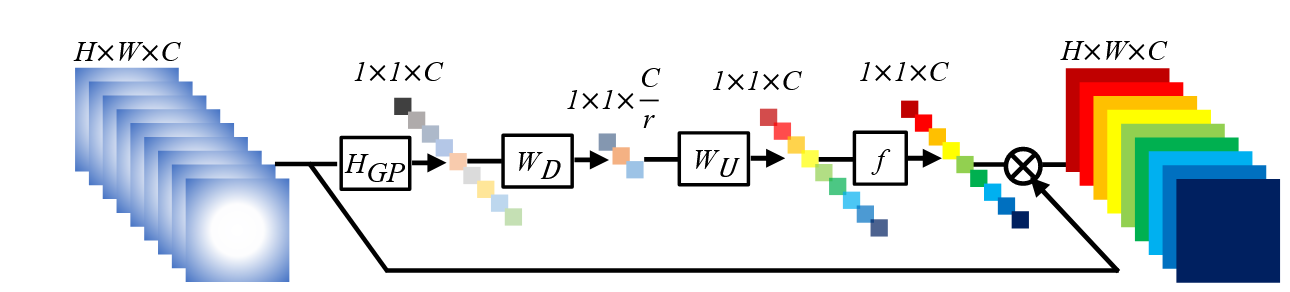
\includegraphics[width=0.9\textwidth]{models/sisr/imgs/channel_attention.png}
    \caption{Image taken from \cite{zhangImageSuperResolutionUsing2018}, Channel Attention machanism.}
    \label{fig:channel_attention}
\end{figure}

The channel attention mechanism depicted in \ref{fig:channel_attention}.
The information of a feature map is first condesated into a single value by using global pooling

    $$z_c = H_{GP}(x_{c}) = \frac{1}{HW} \sum_{i=1}^H \sum_{j=1}^W x_{c}(i, j) ~, $$

with the input $X = [x_1, ..., x_C] \in \mathbb R^{C \times H \times W}$.
The vector $z \in \mathbb R^{C}$ is then processed by a two-layer neural network

    $$\Phi = \sigma \circ F(4, 64) \circ \text{ReLU} \circ F(64, 4) ~, $$

the sigmoid activation function is applied at last, 
in order to squash the attention scores into the interval $[0, 1]$.
Channel attention the weights the inputs according to the attention scores

    \begin{equation} \label{eq:ca}
        H_{CA}(X) = \Phi \circ H_{GP} (X) \cdot X ~.
    \end{equation}

